%\documentclass{beamer}
%\usetheme{Pittsburgh} 
\documentclass{scrartcl}

\usepackage[utf8]{inputenc}
\usepackage{default}
\usepackage[procnames]{listings}
\usepackage{graphicx}
%\usepackage[toc,page]{appendix}
\usepackage{caption}
\usepackage{hyperref}
\usepackage{color}
\usepackage{csvsimple}


%Bibliogrpahy?
%\usepackage{bibentry}
%\nobibliography*
%\bibentry{ }


%Java
\definecolor{javared}{rgb}{0.6,0,0} % for strings
\definecolor{javagreen}{rgb}{0.25,0.5,0.35} % comments
\definecolor{javapurple}{rgb}{0.5,0,0.35} % keywords
\definecolor{javadocblue}{rgb}{0.25,0.35,0.75} % javadoc
\lstset{language=Java,
    basicstyle=\ttfamily,
    keywordstyle=\color{javapurple}\bfseries,
    stringstyle=\color{javared},
    commentstyle=\color{javagreen},
    morecomment=[s][\color{javadocblue}]{/**}{*/},
    breaklines = true,
    columns=fullflexible,
    %Numbering and tabs
    %numbers=left,
    %numberstyle=\tiny\color{gray},
    %stepnumber=2,
    %numbersep=1em,
    tabsize=4,
    showspaces=false,
    showstringspaces=false}

\begin{document}

\title{Manual motion observation}
\subtitle{Assignment No. 1}
\author{
  Matin, Maryam \\
  Quignon, Christophe
  %Familyname, Name
} 
\date{\today}


\maketitle



\section{Experimental setup}
\subsection{Robot Design}
%especially how you mark the stop position and how you ensure identical start positions.
We choose to use the "\href{http://www.damienkee.com/home/2011/8/20/domabot-classroom-robot-design.html}{Domabot}" design (see Figure~\ref{fig:front_view}) in order to minimize the measurement errors. This design has several advantages in this regard:
\begin{itemize}
\item The Motors are directly attached to the brick. Thus the points where distortion can happen are minimized.
\item The center of gravity is very low which increases stability.
\item The track width is big which also increases stability.
\item The free running wheel (see Figure~\ref{fig:free_wheel}) is rigid and quite narrow. Thus it adds less error by friction or deformation.
\end{itemize}

To mark the endpoints of our measures, we designed a pen holder  (See Figure~\ref{fig:pen}) that could adapt to pen size, and be flipped up and down (See Figure~\ref{fig:pen_position}) to not hinder the movement.

\begin{figure}
 \center
 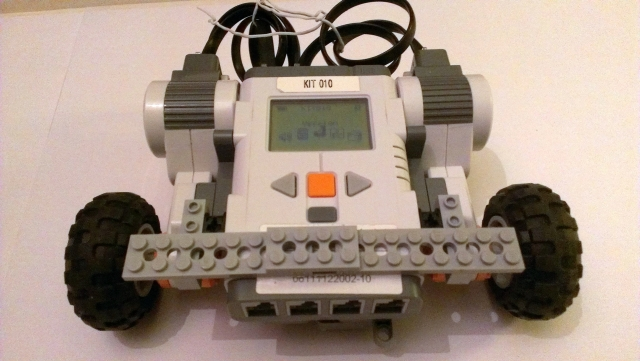
\includegraphics[width= 8cm]{img/robot_front.jpg}
 \caption{The Domabot in front view without pen.}
 \label{fig:front_view}
\end{figure}

\begin{figure}
 \center
 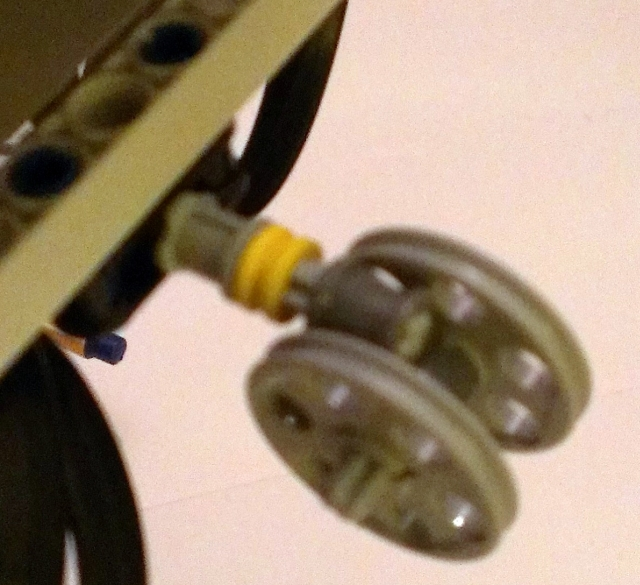
\includegraphics[width= 8cm]{img/steering_wheel.jpg}
 \caption{Detail view of the free wheel}
 \label{fig:free_wheel}
\end{figure}


\section{The program}

The program at its core uses the \texttt{
\href{http://www.lejos.org/nxt/nxj/api/lejos/robotics/navigation/DifferentialPilot.html}{lejos.robotics.navigation.DifferentialPilot}} and two of its functions: \texttt{travel(distance)} and \texttt{travelArc(-radius, distance)}. For convenience we added some structure that allows us to select the direction to drive with the buttons on the robot without the need to restart the program.

\subsection{Program Parameters}
\begin{itemize}
\item wheelDiameter = 5.6f\\
A wheel diameter is specified as 5.8cm in the Handbook and on the wheel itself.

\item trackWidth = 17.6f\
The track width of the robot, measured in cm.

\item distance = 90.0\\
The distance the robot aims to dive in cm.

\item radius\\
 = $250 * \pi \ 180 * 90 = 392.699$\\
 We decided to go with an angular description of the arc in degree for better understanding and a more meaningful tuning. The function needs a radius in cm as input, but we kept the calculation in the code and thus documented best.

\item Delay.msDelay(500)\\
The direction of turn is selected by pushing a button. Before starting the movement, we wait for half a second, so the operator can remove the finger and the robot can recover from the push.
\end{itemize}


\subsection{Code}
(See DiffDrv.java)
\lstinputlisting[language=Java]{DiffDrv.java}


\section{Execution}
After writing and tuning the program we set up the execution in several steps:
\begin{itemize}
\item Load the robots battery to a maximum.
\item Tape together the two sheets of paper on the back side to they perfectly meet without gap or overlap.
\item Tape down the sheets to the ground so they can not move.
\item Put the robot in its starting position.
\item Draw a starting box around the robots shadow (fixed light source) to mark the starting position.
\item Calibrate the pen to touch the paper vertically (See Figure~\ref{fig:pen_calib})
\item Start the program
\item Perform each run:
\begin{enumerate}
	\item Raise the pen
	\item Set the robot to starting position by aligning its shadow (See Figure~\ref{fig:setup})
	\item Align free running wheel along the robots main axis
	\item Select the driving direction with the buttons
	\item Wait for the robot to execute
	\item Lower the pen to mark its arrival position
\end{enumerate}
\end{itemize}

\begin{figure}
 \center
 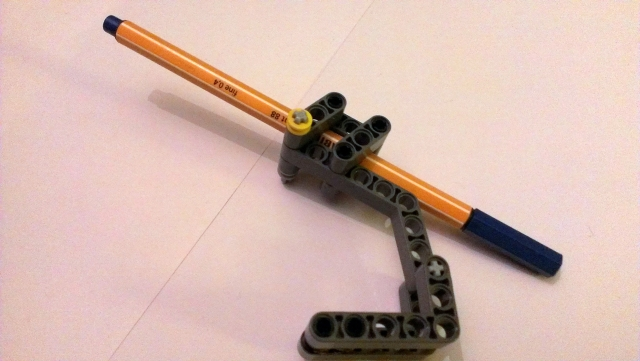
\includegraphics[width= 8cm]{img/pen.jpg}
 \caption{Detail view of the pen holder}
 \label{fig:pen}
\end{figure}

\begin{figure}
\centering
\begin{minipage}{.5\textwidth}
  \centering
  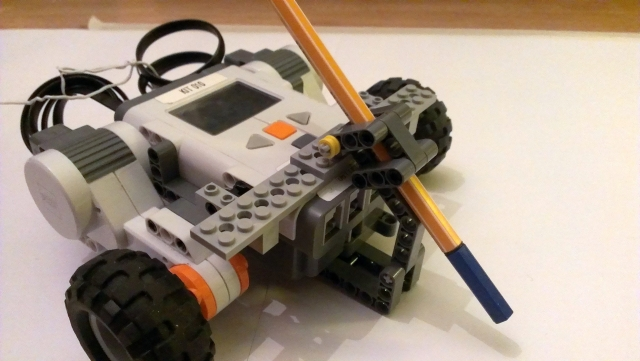
\includegraphics[width=.8\linewidth]{img/pen_up.jpg}
\end{minipage}%
\begin{minipage}{.5\textwidth}
  \centering
  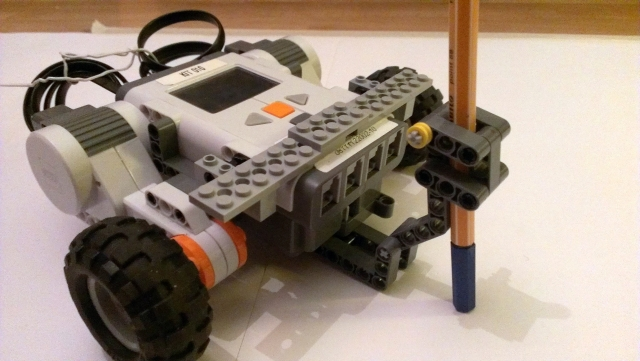
\includegraphics[width=.8\linewidth]{img/pen_down.jpg}
  
\end{minipage}
\caption{The two pen positions of the robot.}
\label{fig:pen_position}
\end{figure}

\begin{figure}
 \center
 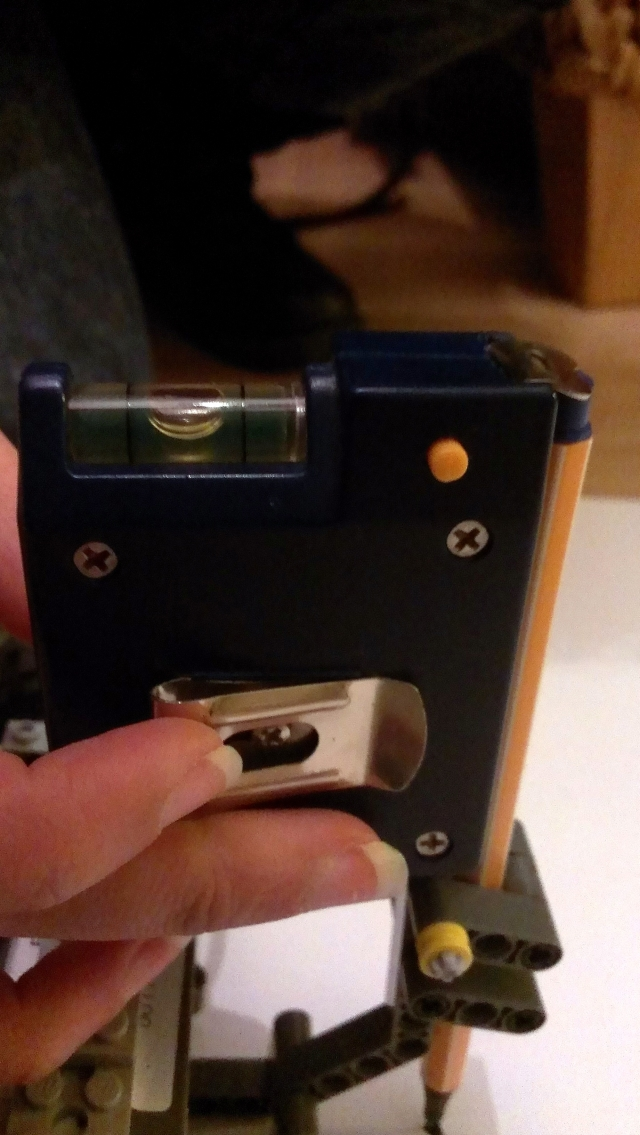
\includegraphics[width= 4cm]{img/pen_adjust.jpg}
 \caption{Calibration of the pen}
 \label{fig:pen_calib}
\end{figure}

\begin{figure}
 \center
 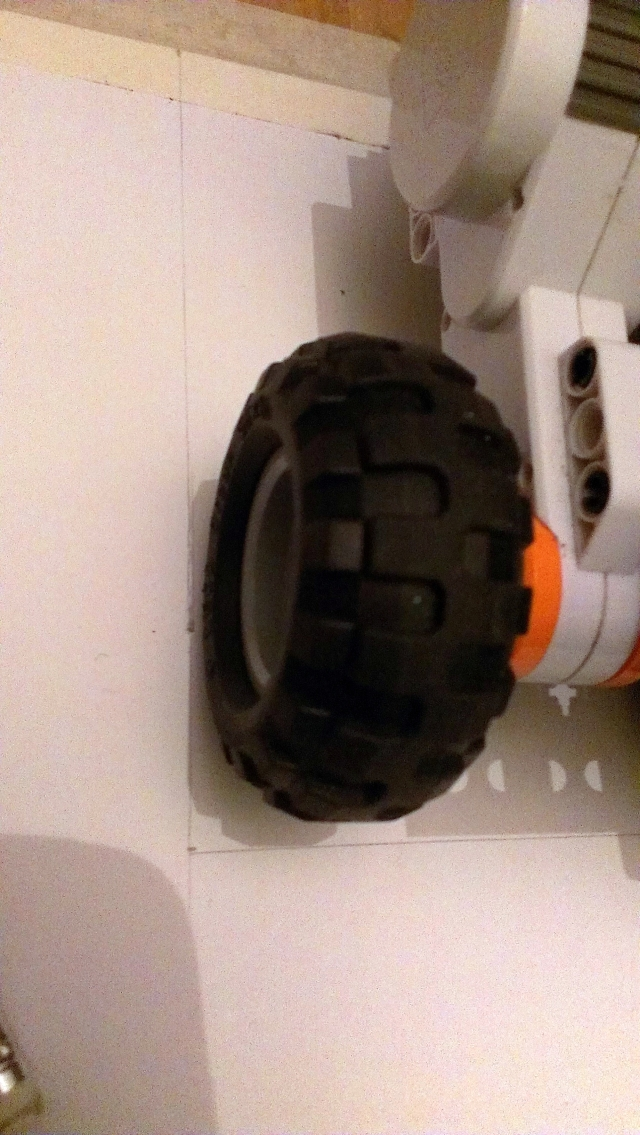
\includegraphics[width= 4cm]{img/wheel_adjust.jpg}
 \caption{The starting position of the Domabot with the help of its shadow.}
 \label{fig:setup}
\end{figure}



\begin{itemize}
\item
\end{itemize}


\section{Observations}
\subsection{Execution}

We run 20 points on each direction. First ahead, then left then right. The points showed up without any pattern and no particular order. But there was, as expected a visible difference in the spread for every direction.\\
In the last third of the 16\textsuperscript{th} run while going to the left, the right wheel came off the axis of the robot (See Figure~\ref{fig:failure}).
We marked the landing position, as it was far off the point cloud up to that point to render it as a failure during the analysis. We fixed the wheel back on the axis and continued the experiment. All following points were also marked but showed no extraordinary spread. To end up with 20 measurement without the failure, we added one more.

\begin{figure}
 \center
 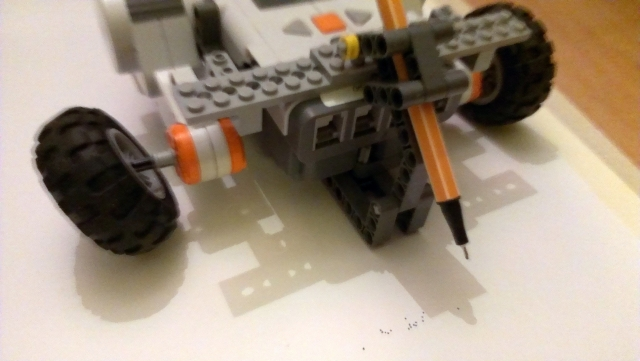
\includegraphics[width= 8cm]{img/wheel_failure.jpg}
 \caption{Image of the wheel failure}
 \label{fig:failure}
\end{figure}

\subsection{Accuracy}
%including how you arrived at these estimates and why they are plausible.
\begin{itemize}
\item
\end{itemize}

\subsection{Precision}
%including how you arrived at these estimates and why they are plausible.
\begin{itemize}
\item
\end{itemize}


\subsection{Measurement}
%TERMS:
%as on slide 14 and 16
\begin{itemize}
\item Measurand:
\item Measurement:
\item Measurement range:
\item Suppression rate:
\item Measurement result:
\item Device Under  Test (DUT): 
\item Measuring System:
\item Measuring principle
\item Measuring Method:
\item Sensitivity:
\end{itemize}
%Measurand


\section{Data}
\subsection{Measured points for the driving ahead.}
 (See data\_ahead.csv)\\
\csvautotabular[separator=semicolon]{data_ahead.csv}

%\begin{figure}
% \center
% \includegraphics[width= 8cm]{img/plot_left.jpg}
% \caption{Plot of the measurements of the left arc.}
% \label{fig:data_left}
%\end{figure}

\subsection{Measured points for the driving to the left.}
 (See data\_left.csv)\\
\csvautotabular[separator=semicolon]{data_left.csv}
%\begin{figure}
% \center
% \includegraphics[width= 8cm]{img/plot_right.jpg}
% \caption{Plot of the measurements of the right arc.}
% \label{fig:data_right}
%\end{figure}

\subsection{Measured points for the driving to the right.}
 (See data\_right.csv)\\
\csvautotabular[separator=semicolon]{data_right.csv}

%\begin{figure}
% \center
% \includegraphics[width= 8cm]{img/plot_ahead.jpg}
% \caption{Plot of the measurements of movement ahead.}
% \label{fig:data_ahead}
%\end{figure}

\section{Summary}
\begin{itemize}
\item
\end{itemize}


%CONTENTS
%NOTES


%COPY AND PASTE FROM HERE

%\begin{enumerate}
% \item 
%\end{enumerate}

%\href{link}{text}

%\begin[Language=Python]{lstlisting}
%#PYTHON CODE HERE
%\end{lstlisting}

%\lstinputlisting[language=Java]{ }

%\csvautotabular[separator=semicolon]{data.csv}

%\begin{figure}
% \center
% \includegraphics[width= cm]{img/ }
% \caption{}
%\end{figure}

%BIBLIOGRPAHY?
\bibliographystyle{plain}%amsalpha
\bibliography{Top30.bib}
%\bibentry{}

\end{document}
